\documentclass[compress,notes=hide]{beamer}
\usetheme[height=10mm]{Rochester} 
%\usefonttheme[onlymath]{serif}
\xdefinecolor{lavendar}{rgb}{0.29,0.43,0.52}
\usecolortheme[named=lavendar]{structure}
\setbeamertemplate{items}[ball] 

\usepackage[noend]{algpseudocode}
\usepackage{amsmath}
\usepackage{amsthm}
\usepackage{cancel}
\usepackage{rotating}
%\newtheorem{theorem}{Theorem}
%\newtheorem{lemma}{Lemma}
\newtheorem{algorithm}{Algorithm}
\newtheorem{defn}{Definition}
\newcommand\proda[1]{\displaystyle\prod_{#1}}
\newcommand\prodb[2]{\displaystyle\prod_{\stackrel{{#1} :}{#2}}}
\newcommand\prodc[1]{\prod_{#1}}
\newcommand\prodd[2]{\prod_{#1}^{#2}}
\newcommand\suma[1]{\displaystyle\sum_{#1}}
\newcommand\sumb[2]{\displaystyle\sum_{\stackrel{{#1} :}{#2}}}
\newcommand\sumc[1]{\sum_{#1}}
\newcommand\sumd[2]{\sum_{#1}^{#2}}

\newcommand\blue[1]{\structure{\textit{#1}}}

\newcommand\ignore[1]{}

\title{Cooperative Coevolution and Univariate Estimation of Distribution Algorithms}
\author{Christopher Vo$^1$ \and Liviu Panait$^2$ \and Sean Luke$^1$}
\institute{
  $^1$Department of Computer Science\\
  George Mason University\\
  Fairfax, VA, USA\\
  \quad\\ 
  $^2$Google, Inc.\\
  Santa Monica, CA, USA
}
\date{FOGA 2009}

\begin{document}

%==========================================================%
% The abstract slide for this presentation 

\frame{\titlepage

\note{
\begin{itemize}
\item I am presenting a relationship we have identified between Cooperative Coevolutionary Algorithms (CCEAs) and Estimation of Distribution Algorithms (EDAs).\newline
\item We believe that this interesting relationship may permit \blue{cross pollination} between the two fields.
\end{itemize}
}
}

%==========================================================%

\section[Outline]{}
\frame{
\frametitle{Outline} 

%\tableofcontents

\structure{Cooperative Coevolutionary Algorithms (CCEAs)}
\begin{itemize}
\item Evolutionary Game Theory CCEA Model
\item Some Prior Work in CCEAs
\end{itemize}

\vfill\structure{Estimation of Distribution Algorithms (EDAs)}
\begin{itemize}
\item Univariate/Bivariate/Multivariate EDAs
\item Population-Based Incremental Learning (PBIL)
\end{itemize}

\vfill\structure{CCEAs \(\longleftrightarrow\) EDAs}


\vfill\structure{An Example of Cross-Pollination }
\begin{itemize}
\item A Theoretical EDA with Convergence Properties
\item A Real Approximation to the Theoretical EDA
\item Empirical Analysis
\end{itemize}

\vfill\structure{Conclusions and Future Work }

\note{
\begin{itemize}
\item First, we're going to talk about relevant work in the field of CCEAs. In particular, a model of CCEAs based on Evolutionary Game Theory.
\item Then we'll talk about EDAs and their various forms, including a particular univariate EDA called Population-based Incremental Learning (PBIL)
\item We will show that CCEAs and Univariate EDAs are essentially the same thing.To demonstrate this, we take a CCEA and show the equivalent EDA.
\item Then we:
\begin{itemize}
\item Prove that the theoretical algorithm has convergence properties.
\item Present an implementation of this algorithm.
\end{itemize}
\end{itemize}
}
}

%==========================================================%
% An quick overview of CCEAs

\section{Cooperative Coevolution}

\subsection{Overview}

\frame{
\frametitle{Coevolution}
\vspace{-1em}
\begin{block}{Idea}
The relative ordering between two individuals is based in part on the presence of other individuals in the system. 
\end{block}
\vspace{0.5em}
{\bf Major Coevolutionary Frameworks:}\newline
\begin{itemize}
\item One-population competitive
\begin{itemize} 
	\item Checker players (Chellapilla and Fogel, 1999)\newline
\end{itemize}
\item Two-population competitive
\begin{itemize}
	\item Sorting networks versus sorting problems (Hillis, 1991)\newline
\end{itemize}
\item \(N\)-population cooperative (Potter and De Jong, 1994, 2000)
\begin{itemize}
	\item e.g. Heterogeneous behaviours for players on a soccer team
\end{itemize}
\end{itemize}

\note{\footnotesize{(We realize that there is some ``discussion'' about these terminologies and definitions, but this is what we're going with.) We believe that the \blue{fundamental dynamic} in coevolution is that the relative ordering between two individuals depends in part on the presence of other individuals in the system.\newline

There are three major types of coevolution:
\begin{itemize}
	\item {\bf 1-pop competitive:} An ordinary 1-population system except that the fitnesss is based on the context of other individuals competing from the same population. This is common when you have game-playing individuals, for example, and it's hard to define a good fitness procedure.
	\item {\bf 2-pop competitive:} Involve another population that acts as a ``foil''. Notionally, you {\it might} use 2-pop when you want to develop a robust solution, such as in the classic example of evolving sorting algorithms by pitting them against sorting problems. 
	\item {\bf \(N\)-pop cooperative (CCEA):} Our work concentrates on this type. (Jump to next slide)
\end{itemize}
}
}

}

\frame{
\frametitle{Cooperative Coevolutionary Algorithms (CCEAs)}
\begin{center}
\includegraphics[width=0.85\textwidth]{coevolution.pdf}
\end{center}

\note{
This is what we're going with as an example of a CCEA: 
\begin{itemize}
\item Decompose the solution space into \(N\) subsolution spaces, giving each its own population. 
\item To asssess the fitness of an individual, group with individuals of the other populations, incorporate joint fitness into the individual's fitness.
\item It's {\it cooperative} in the sense that an individual's fitness is based in part on how well he worked with them. 
\end{itemize}
}
}

%==========================================================%
% An overview of prior work in CCEAs

\subsection{Prior Work in CCEAs}
\frame{
\frametitle{Relevant Results from CCEAs}
\vspace{-0.8em}
\begin{itemize}
\item \textbf{Investigation of CCEAs with an EGT-based model}\newline(Wiegand, 2003) \newline
\item \textbf{Relative Overgeneralization}\newline(Wiegand, 2004)\newline
\item \textbf{Convergence using Max fitness}\newline(Panait, 2006) \newline
\item \textbf{Convergence using Max-of-N fitness}\newline(Panait, Tuyls, and Luke, 2008) \newline
\item \textbf{Archive Methods}\newline(Bucci and Pollack, 2005; Panait, Luke, and Harrison 2006) 
\end{itemize}

\note{There has been substantial work in cooperative coevolution.  In the next few slides, I'll present some of the results that are relevant to our work. 

\begin{itemize}
\item Leading up to this, an example of Wiegand's infinite population model of CCEAs using a well-known Evolutionary Game Theory model.
\item Then, a widely observed pathology in cooperative algorithms called Relative Overgeneralization,
\item Later it was found that the system will converge to the global optimum when a particular fitness aggregation mechanism (the maximum) is used
\item That convergence was then extended using a subset \(N\) collaborators to estimate the maximum 
\item And methods of determining what that subset should be (Archive Methods)
\end{itemize}
}
}

%==========================================================%
% We describe EGT CCEA model

\subsection{EGT CCEA Model (Wiegand, 2003)}
\frame{
\frametitle{A Cooperative Coevolution EGT Model}
\textbf{\structure{Some assumptions and representation:}}\newline
\begin{itemize}
\item {\bf Two Infinite} populations, with \textbf{Finite} sets of genotypes\newline
\item {\bf Population 1:}{\hfill}Vector $x$ where $x_i$ is proportion of genotype $i$.\newline
{\it and}{\hfill}Vector $u$ where $u_i$ is the fitness of genotype $i$.\newline
\item {\bf Population 2:}{\hfill}Vector $y$ where $y_j$ is proportion of genotype $j$.\newline 
{\it and}{\hfill}Vector $w$ where $w_i$ is the fitness of genotype $j$.\newline
\item {\bf Reward matrix:} $A: a_{ij}$ is reward when $i$ and $j$ are combined.\newline
\item {\bf Cooperative}: \(A = A^T\)
\end{itemize}
}



\frame{
\frametitle{CCEA EGT Model (Wiegand, 2003)}
\textbf{\structure{Procedure:}}
\begin{enumerate}
\item Assess fitness ({\it complete mixing:} average over all collaboration in opposing population)
\begin{align*}
u_i^{(t)} &= \sum_j a_{ij} y_j^{(t)} &
w_j^{(t)} &= \sum_i a_{ij} x_i^{(t)}
\end{align*}
\item Update genotype proportions (via fitness-proportional selection)
\begin{align*}
x_i^{(t+1)} &= x_i^{(t)} \left( \frac{u_i^{(t)}}{\sum_k x_k u_k^{(t)}} \right) &
y_j^{(t+1)} &= y_j^{(t)} \left( \frac{w_j^{(t)}}{\sum_k y_k w_k^{(t)}} \right)
\end{align*}
\end{enumerate}

\note{
One particular CCEA EGT model by Wiegand is broken into two parts, where assess the fitness and then update the genotype proportions. 

Wiegand's model assesses fitness using a ``complete mixing'' model --- the average over all collaborations in the opposing population. Let \(u_i\) represent the fitness of genotype \(i\) in population 1 and \(w_j\) be the fitness of genotype \(j\) in population 2; The fitness is computed in this way. \newline

The update step models fitness proportional selection.  
}
}

\frame{
\frametitle{Relative Overgeneralization (Wiegand, 2004)}
\blue{Averaging over all collaborations} leads to convergence to local suboptima surrounding Nash equilibria in the joint space.

\vspace{2em}
{\it \small Two-Peaks\\
Problem}
\vspace{-4em}\begin{center}
\includegraphics[width=0.80\textwidth,trim=0 0 0 1.8in]{twopeaks.pdf}
\end{center}


\note{
One pathology that is widely observed in CCEAs is relative overgeneralization --- fittest individuals tend to be those that perform well with the average collaborator rather than with the optimal collaborator. This can be illustrated by the following depiction of\newline

{\bf Figure:} The classic \blue{two peaks problem}. A joint fitness landscape \(f(i,j)\) in the CCEA. Suboptimal peak with wide coverage, optimal peak with narrow coverage. Both peaks are \blue{Nash equilibria}. \newline

For a genotype \(i\), near the low, wide peak, there are exist many strategies that perform well relative to \(i\). If \(i\) is near the high peak, there are some strategies that do extremely well --- but it may not perform very well on average.\newline

So when the fitness is computed as the average, the system will collect at the suboptimal peak.  
}
}



%==========================================================%
% We describe convergence using max & tournament selection from Liviu

\frame{
\frametitle{Convergence Using Max Fitness (Panait, 2006)}
System will converge to the global optimum if fitness is assessed as the \blue{maximum over all collaborations}.
\vspace{-0.2em}
\begin{align*}
u_i^{(t)} & = \max_j a_{ij} &
w_j^{(t)} &= \max_i a_{ij}
\end{align*}

Update procedure (modeling tournament selection of size \(H\)):
\begin{align*}
x_i^{(t+1)} &= x_i^{(t)} \frac{\left(\sum_{\forall k : u_k^{(t)} \leq u_i^{(t)}} x_k^{(t)} \right)^H \!\!\! - \left( \sum_{\forall k : u_k^{(t)} < u_i^{(t)}} x_k^{(t)} \right)^H} {\sum_{\forall k : u_k^{(t)} = u_i^{(t)}} x_k^{(t)}} \\
\\
y_i^{(t+1)} &= y_j^{(t)} \frac{\left( \sum_{\forall k : w_k^{(t)} \leq w_j^{(t)}} y_k^{(t)} \right)^H \!\!\!\! -\left( \sum_{\forall k : w_k^{(t)} < w_j^{(t)}} y_k^{(t)} \right)^H}{\sum_{\forall k : w_k^{(t)} = w_j^{(t)}} y_k^{(t)}} \\
\end{align*}


\note{
Later, Panait provided a proof of convergence if the fitness is based on the maximum over all collaborations. With more accurate estimates of the maximum, less drift towards suboptimal solutions occurs. \newline

\footnotesize{
(if needed) This curious equation is a result of the order statistics to compute the expected maximum over a set of size \(H\).  
\begin{itemize}
\item In each subequation there are two terms raised to \(H\) each.  The numerator the probability that, of a tournament of size \(H\), the winners (there may be ties) will include a genotype whose fitness is the same as genotype \(i\).
\item The first term gives the probability that all \(H\) tournament entrants will have a fitness less than or equal to \(i\)'s fitness, and the second term gives the probability that all will have a fitness less than that of \(i\).  
\item The denominators in each subequation compute the probability that the first such winner is in fact \(i\), as opposed to other fitness-equivalent genotypes.
\end{itemize}
}
}
}


\frame{
\frametitle{Max-of-N (Panait et al, 2008)}
A weakened convergence proof when the max is taken as an estimate over \blue{N collaborators} instead of all collaborators.  Fitness assessment now:
\[
\begin{split}
u_i^{(t)} &= \sum_j a_{ij} y_j^{(t)} \frac{\left( \sum_{\forall k : a_{ik} \leq a_{ij}} y_k^{(t)} \right)^N \!\!\! -\left( \sum_{\forall k : a_{ik} < a_{ij}} y_k^{(t)} \right)^N} {\sum_{\forall k : a_{ik} = a_{ij}} y_k^{(t)}} \\
w_i^{(t)} &= \sum_i a_{ij} x_i^{(t)} \frac{\left( \sum_{\forall k : a_{kj} \leq a_{ij}} x_k^{(t)} \right)^N \!\!\! - \left( \sum_{\forall k : a_{kj} < a_{ij}} x_k^{(t)} \right)^N} {\sum_{\forall k : a_{kj} = a_{ij}} x_k^{(t)}} \\
\end{split}
\]

Update procedure: still tournament selection.


\note{Panait found that instead of using the expected maximum, it is possible to use an estimate over \(N\) randomly chosen collaborators.

As you can see, this looks similar to the update procedure ---

Question: How to determine \(N\)?
}

}

%==========================================================%
% We describe Max-of-N tournament selection epsilon proof from Liviu

\frame{
\frametitle{Empirical Demonstration of Max-of-N}
\vspace{-1em}\begin{center}
%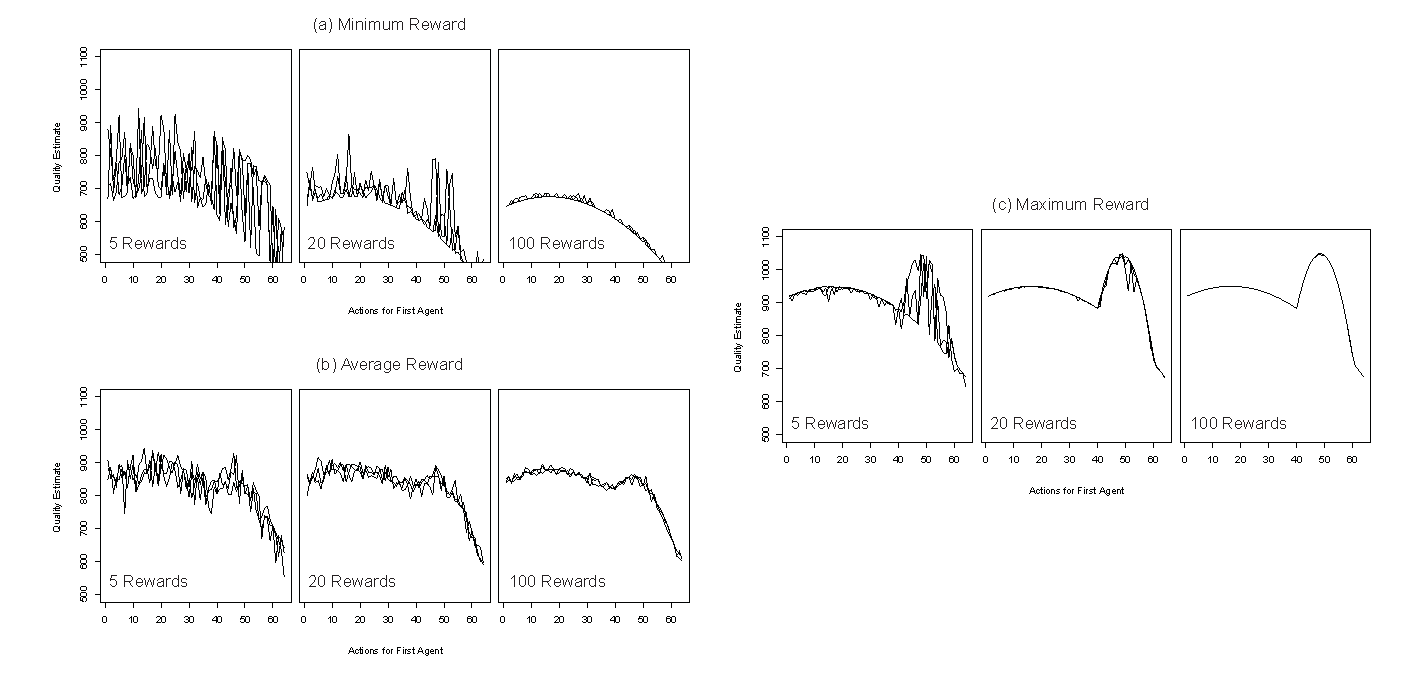
\includegraphics[width=\textwidth]{maxcollaborator.pdf}
\hspace{-0.5em}\begin{rotate}{90}{~~~~~~~~~Maximum-of-N}\end{rotate}\hspace{0.5em}\includegraphics[width=\textwidth]{maxliviu.pdf}\\
\hspace{-0.5em}\begin{rotate}{90}{~~~~~~~~~Average-of-N}\end{rotate}\hspace{0.5em}\includegraphics[width=\textwidth]{averageliviu.pdf}
\end{center}
\note{

Question: How to determine \(N\)?
}

}





%==========================================================%
% We describe Archive Methods

\frame{
\frametitle{Archive Methods} 
\begin{block}{Archive} A subset of individuals from the collaborating population(s) which provides as good an assessment as testing against the entire set of collaborators would provide.\end{block}
\vspace{1em}
{\bf Examples:}
\vspace{0.5em}
\begin{itemize}
\item Pareto-dominance mechanism in pCCEA \\(Bucci and Pollack 2005).\newline

\item Using rank ordering \\ (Panait, Luke, and Harrison 2006).
\end{itemize}

\note{
Bucci: Identifying the front of pareto-nondominated candidates for individuals in the alternate population. \newline

Panait/Luke: Identifying individuals which, when used for comparison, change the rank order of the opposing population
}
}

%==========================================================%
% We describe miscoordination

%\frame{
%\frametitle{Miscoordination}
%Selecting an optimal individual in one population is no guarantee that optimal %actions will be selected in others. The penalties caused by miscoordination can %significantly slow down convergence.
%}

%==========================================================%
% We describe EDAs

\section{Estimation of Distribution Algorithms}


\frame{
\frametitle{Estimation of Distribution Algorithms (EDAs)}
\vspace{-0.5em}
\begin{block}{Idea:}
Replace the population model with a statistical distribution of the space.\\
\end{block}
\vspace{1em}
Problem 1: It's challenging to represent a high-dimensional space
\begin{itemize}
\item Project the distribution into {\it per-gene} marginal distributions (Univariate EDAs), losing data
\item Attempt to capture higher-order distributions (Bivariate, Multivariate EDAs)
\end{itemize}

Problem 2: How to model the distribution?
\begin{itemize}
\item Multi-modal, real-valued distributions?
\item Representations as Trees? Lists? Sets? Graphs?  
\end{itemize}

\note{Now we switch to the relevant work in Estimation of Distribution Algorithms. In a typical evolutionary algorithm, you sample from a population. For EDAs, on the other hand, replace the notion of a population with a statistical distribution of the space.\newline 
}
}

\frame{
\frametitle{Examples of EDA Models}

\begin{itemize}
\item {\bf Univariate Models} model each variable independently. 
\begin{itemize}
	\item PBIL (Baluja, 1995)
	\item UMDA (M\"uhlenbein and Paa\ss{}, 1996)
	\item Compact GA - cGA (Harik, Lobo, Goldberg 1998) \newline
\end{itemize}
\item {\bf Bivariate Models} capture pairwise or second-order interactions.
\begin{itemize}
	\item COMIT (Baluja, Davies 1997)
	\item MIMIC (DeBonet 1996) \newline
\end{itemize}
\item {\bf Multivariate Models} model complex interactions and higher-order interactions.
\begin{itemize}
	\item BOA (Pelikan, Goldberg, Cant\'u-Paz, 1998)
	\item Hierarchical BOA (Pelikan and Goldberg, 2000)
\end{itemize}
\end{itemize}


\note{
There are many notable EDA models.
\footnotesize{
\begin{itemize}
\item For example, to model very simple or no interactions between variables, you can use univariate models such as PBIL, UMDA, and the Compact Genetic Algorithm (CGA). 
\item There are also many examples of more complex models such as bivariate models, that capture pairwise interactions (examples of which are COMIT and MIMIC), and
\item Multivariate models such as the widely known Bayesian Optimization Algorithm (BOA) which are perhaps capable of capturing higher-order interactions. 
\end{itemize}
}
\tiny{
\begin{itemize}
\item PBIL: After generating a number of solutions the very best solutions are selected and the probability vector is shifted towards the selected solutions by using Hebbian learning rule

\item CGA: Update Rule: Each component of the vector is updated by shifting its value by the contribution of a single individual to the total frequency assuming a particular population size \(k\). 

\item UMDA: Select \(N\), throw away the other \(N-1\). Compute histogram for each gene. Use the new distribution to generate another \(N-1\) solutions.
\end{itemize}
}
}
}


\frame{
\frametitle{Population-Based Incremental Learning (Baluja, 1994)}
\vspace{-1em}
\begin{block}{Definitions for PBIL:}
\begin{itemize}\small{
\item \textbf{Individuals:} Boolean vector \(i=\lbrace 0,1\rbrace^G\)
\item \textbf{Probability distribution:} Vector \(D\); \(D_g\) is probability that \(i_g=1\).
\item \textbf{Population Size:} \(Q\), \textbf{Selection Size:} \(R\)
\item \textbf{Learning Rate:} \(\alpha\)}
\end{itemize}
\end{block}
\small{
\begin{algorithmic}[0]
\Loop \hspace{\fill} 
	\For{q from 1 to Q}
		\State Sample individual \(i_q\) from \(D\).
		\State Evaluate(\(i_q\))
	\EndFor
	\State Select the best \(R\) individuals from among \(i_1...i_Q\)
	\For{each gene \(g\)}
		\State Let \(N_g\) be the distribution of alleles for \(g\) among
		\State \quad the \(R\) best individuals
		\State Update gene distribution \(D_g \leftarrow (1-\alpha) D_g + \alpha N_g\)
	\EndFor
\EndLoop
\end{algorithmic}
}

\note{I'd like to highlight a particular Univariate EDA that we have used in our work: Population-Based Incremental Learning (PBIL). \newline

(Go through slide materials)\newline

Essentially you:
\begin{itemize}
\item Repeatedly sample and evaulate inviduals from D to create a population of size Q. 
\item Then you select R of the best solutions and 
\item Shift the probability vector towards the selected solutions using the update rule shown.
\end{itemize}
}}


%==========================================================%
% We describe relationship between CCEAs and EDAs
% TODO discuss "real ccea" vs "egt ccea"
% TODO discuss how there are things that you can do with samples
%   that you can't do with a univariate EDA?

\frame{
\frametitle{Relationship between CCEA and EDA}
\blue{The EGT model for CCEAs is a Univariate EDA!}
\newline

\begin{itemize}
\item Each population in the EGT CCEA model is represented by a set of proportions of each genotype.\\
\vspace{0.5em}
Selections from each population are formed to create a joint solution.

\vspace{1em}
\item Each variable in a Univariate EDA is represented by a separate distribution (which can also be represented by a set of proportions).\\

\vspace{0.5em}
Selections from each distribution are formed to create a joint solution.
\end{itemize}

\note{ 
So now that we've given some detail about CCEAs and EDAs, we return to the thesis of our work. First, the relationship between EGT CCEA model and the Univariate EDAs is apparent by observing that \newline

(point to slides)\newline

However, note the EGT CCEA model so far has considered only two populations...
In our work, we show that the proof still holds for EGT CCEAs. 
}
}


\frame{
\frametitle{A CCEA-inspired Theoretical EDA}
\begin{theorem}
Given a joint reward system with a unique global optimum $a_{i_1^\star i_2^\star ... i_M^\star}$, for any $\epsilon > 0$ and any $H \geq 2$, there exists a value $N_\epsilon \geq 1$ such that the theoretical CCEA model converges to the global optimum with probability greater than $\left(1-\epsilon\right)$ for any number of collaborators $N \geq N_\epsilon$.\end{theorem}
}


%==========================================================%
% We describe the proof by Panait. 

\frame{
\frametitle{Proof Notation}
\(X_p\): The space of genotypes of population \(p\).\newline

\(X_{-p}\): The joint space of collaborators for an individual from population \(p\).\newline

\({_p}x^{(t)}_i\): Ratio of individuals with genotype \(i\) for population \(p\) at generation \(t\). \newline

\(j\): A tuple of genotypes chosen to collaborate with \(i\).\newline

\(y_j\): The proportion of collaborating tuple \(j\) in the joint space.\newline

\(a_{ij}\): The reward received for genotype \(i\) when combined with collaborators described by tuple \(j\).

\note {
Note the EGT CCEA model so far has considered only two populations...
In our work, we show that the proof still holds for EGT CCEAs. 
}
}

% 0: EGT CCEA Model
\frame{
\frametitle{Revised EGT CCEA Model for \(N\) Populations}
Fitness of genotype \(i\) in population (distribution) \(p\) at time \(t\) (maximum of \(N\) evaluations):
\noindent\begin{eqnarray*}
{_p}u^{(t)}_i & \!\!\!\!= &\!\!\!\! \suma{j \in X_{-p}} { a_{i j} \frac{y^{(t)}_j}{\sumb{k \in X_{-p}}{a_{i k} = a_{i j}} y^{(t)}_k} \left( \left( \sumb{k \in X_{-p}}{a_{i k} \leq a_{i j} } y^{(t)}_k \right)^N - \left( \sumb{k \in X_{-p}}{a_{i k} < a_{i j} } y^{(t)}_k \right)^N \right) } \label{approx_eqn1}\\
\end{eqnarray*}

Population proportion update for genotype \(i\) in population (distribution) \(p\) at time \(t+1\) (tournament selection of size \(H\)): 
\begin{eqnarray*}
{_p}x^{(t+1)}_i  & \!\!\!\!= &\!\!\!\! \frac{{_p}x^{(t)}_i}{\!\!\!\!\sumb{k}{\!\!\!\!{_p}u^{(t)}_k = {_p}u^{(t)}_i} {_p}x^{(t)}_k} \left( \left( \sumb{k}{{_p}u^{(t)}_k \leq {_p}u^{(t)}_i} {_p}x^{(t)}_k \right)^H - \left( \sumb{k}{{_p}u^{(t)}_k < {_p}u^{(t)}_i} {_p}x^{(t)}_k \right)^H \right) \label{approx_eqn2}
\end{eqnarray*}
\note{
The EGT CCEA Model with N individuals looks like this, which was described earlier. The top equation is a formulation of the Max-of-N fitness evaluation, and the bottom equation is a formulation of tournament selection.
}
}

\ignore{
\frame{
\frametitle{Introducing \(\epsilon\)}
\begin{lemma}
Assume the populations for the EGT model are initialized at random based on a uniform distribution over all possible initial populations.  Then, for any $\epsilon>0$, there exists $\eta_\epsilon>0$ such that

\[
\begin{split}
&P\left( \min_{p=1..M} \min_{i=1..n_p} {_p}x^{(0)}_i > \eta_\epsilon \wedge \max_{p=1..M} \max_{i=1..n_p} {_p}x^{(0)}_i < 1-\eta_\epsilon\right)\\
&\qquad\qquad\geq 1 - \epsilon
\end{split}
\]
\end{lemma}
\note{
First, we introduce $\epsilon$ by saying that for an $\epsilon$ value, there is an arbitrary non-zero probability that the populations contain values that are not too close to 0 or 1. 
}
}
}


% 2: Establish
\frame{
\frametitle{No Non-ideal Individual Can Reach the Optimum (\(> \alpha)\)}
(Of course)
\noindent\begin{eqnarray*}
 {_p}u^{(t)}_{i \neq i^{\star}} & = & \suma{j \in X_{-p}} { a_{i j} \frac{y^{(t)}_j}{\sumb{k \in X_{-p}}{a_{i k} = a_{i j}} y^{(t)}_k} \left( \left( \sumb{k \in X_{-p}}{a_{i k} \leq a_{i j} } y^{(t)}_k \right)^N - \left( \sumb{k \in X_{-p}}{a_{i k} < a_{i j} } y^{(t)}_k \right)^N \right) }\\
& \leq & \suma{j \in X_{-p}} { \alpha \frac{y^{(t)}_j}{\sumb{k \in X_{-p}}{a_{i k} = a_{i j}} y^{(t)}_k} \left( \left( \sumb{k \in X_{-p}}{a_{i k} \leq a_{i j} } y^{(t)}_k \right)^N - \left( \sumb{k \in X_{-p}}{a_{i k} < a_{i j} } y^{(t)}_k \right)^N \right) }\\
& \leq & \alpha \suma{j \in X_{-p}} { \left( \left( \sumb{k \in X_{-p}}{a_{i k} \leq a_{i j} } y^{(t)}_k \right)^N - \left( \sumb{k \in X_{-p}}{a_{i k} < a_{i j} } y^{(t)}_k \right)^N \right) } \leq \alpha
\end{eqnarray*}
\note{
First, let $\alpha$ be the second highest element joint reward. Then if the fitness of genotype i for population p is not the maximum, it must be $<= \alpha$. 

We will return to this later.
}
}

% 3: Proof of lower bound for pui*
\frame{
\frametitle{Lower Bound for the Ideal Individual Given \(N\)}
From the evaluation procedure: 
\begin{eqnarray*}
{_p}u^{(t)}_{i^\star} & \!\!\!\!= & \!\!\!\!\suma{j \in X_{-p}} { a_{i^\star j} \frac{y^{(t)}_j}{ \!\!\!\!\sumb{k \in X_{-p}}{a_{i^\star k} = a_{i^\star j}} \!\!\!\!y^{(t)}_k } \left( \left( \sumb{k \in X_{-p}}{a_{i^\star k} \leq a_{i^\star j} } \!\!\!\!y^{(t)}_k \right)^N \!\!\!\!- \left( \sumb{k \in X_{-p}}{a_{i^\star k} < a_{i^\star j} } \!\!\!\!y^{(t)}_k \right)^N \right) }
\end{eqnarray*}
\note{
Next we show how to find a lower bound for the fitness of best genotype for population $p$. This is simply the evalulation procedure when we use $i*$. 
}
}

\frame{
%\frametitle{Finding lower bound for ${_p}u_{i*}{(t)}$}
\frametitle{Lower Bound for the Ideal Individual Given \(N\)}
Break the fitness sum into (1) rewards with optimal collaborators, (2) negative and non-negative results with non-optimal collaborators.
\begin{eqnarray*}
{_p}u^{(t)}_{i^\star} & \!\!\!\!= & \!\!\!\!a_{i^{\star} j^{\star}} \left( 1 - \left( 1 - y^{(t)}_{j^\star} \right) ^N \right) +\\
& & \!\!\!\!\!\!\!\!\!\!\sumb{j \in X_{-p}}{j \neq j^\star \wedge a_{i^\star j} \geq 0} { \!\!\!\!a_{i^\star j} \frac{y^{(t)}_j}{ \sumb{k \in X_{-p}}{a_{i^\star k} = a_{i^\star j} } \!\!\!\!y^{(t)}_k} \left( \left( \sumb{k \in X_{-p}}{a_{i^\star k} \leq a_{i^\star j} } \!\!\!\!y^{(t)}_k \right)^N \!\!\!\!- \left( \sumb{k \in X_{-p}}{a_{i^\star k} < a_{i^\star j} } \!\!\!\!y^{(t)}_k \right)^N \right) }+\\
& & \!\!\!\!\!\!\!\!\!\!\sumb{j \in X_{-p}}{j \neq j^\star \wedge a_{i^\star j} < 0} { \!\!\!\!a_{i^\star j} \frac{y^{(t)}_j}{ \sumb{k \in X_{-p}}{a_{i^\star k} = a_{i^\star j} } \!\!\!\!y^{(t)}_k} \left( \left( \sumb{k \in X_{-p}}{a_{i^\star k} \leq a_{i^\star j} } \!\!\!\!y^{(t)}_k \right)^N \!\!\!\!- \left( \sumb{k \in X_{-p}}{a_{i^\star k} < a_{i^\star j} } \!\!\!\!y^{(t)}_k \right)^N \right) }
\end{eqnarray*}
\note{
We break this into the sum of three pieces:
\begin{itemize}
\item The situation in which it is collaborating with the optimal tuple.
\item The situations where the reward is $>= 0$.
\item The situations where the reward is $< 0$.
\end{itemize}
}
}

\ignore{
\frame{
\frametitle{Lower Bound for the Ideal Individual Given \(N\)}
\begin{eqnarray*}
{_p}u^{(t)}_{i^\star} & \!\!\!\!\geq & \!\!\!\!a_{i^{\star} j^{\star}} \left( 1 - \left( 1 - y^{(t)}_{j^\star} \right) ^N \right) +\\
& & \!\!\!\!\!\!\!\!\!\!\sumb{j \in X_{-p}}{j \neq j^\star \wedge a_{i^\star j} \geq 0} { \!\!\!\!a_{i^\star j} \frac{y^{(t)}_j}{ \sumb{k \in X_{-p}}{a_{i^\star k} = a_{i^\star j} } \!\!\!\!y^{(t)}_k} \left( \left( \sumb{k \in X_{-p}}{a_{i^\star k} \leq a_{i^\star j} } \!\!\!\!y^{(t)}_k \right)^N \!\!\!\!- \left( \sumb{k \in X_{-p}}{a_{i^\star k} < a_{i^\star j} } \!\!\!\!y^{(t)}_k \right)^N \right) }+\\
& & \!\!\!\!\!\!\!\!\!\!\cancel{\sumb{j \in X_{-p}}{j \neq j^\star \wedge a_{i^\star j} < 0} { \!\!\!\!a_{i^\star j} \frac{y^{(t)}_j}{ \sumb{k \in X_{-p}}{a_{i^\star k} = a_{i^\star j} } \!\!\!\!y^{(t)}_k} \left( \left( \sumb{k \in X_{-p}}{a_{i^\star k} \leq a_{i^\star j} } \!\!\!\!y^{(t)}_k \right)^N \!\!\!\!- \left( \sumb{k \in X_{-p}}{a_{i^\star k} < a_{i^\star j} } \!\!\!\!y^{(t)}_k \right)^N \right) }}
\end{eqnarray*}
\note{
For now, we're not so interested in the negative reward sitaution so we can eliminate it  
}
}

\frame{
\frametitle{Finding lower bound for ${_p}u_{i*}{(t)}$ (continued)}
\vspace{-1em}
\begin{eqnarray*}
{_p}u^{(t)}_{i^\star} & \geq & a_{i^{\star} j^{\star}} - \left( 1 - y^{(t)}_{j^\star} \right) ^N \left( a_{i^{\star} j^{\star}}  - \sumb{j \in X_{-p}}{j \neq j^\star \wedge a_{i^\star j} < 0} { a_{i^\star j} } \right)\\
& \geq & a_{i^{\star} j^{\star}} - \left( 1 - \prodb{r=1..M}{r \ne p} {_r}x^{(t)}_{j_r^\star} \right) ^N \left( a_{i^{\star} j^{\star}}  - \sumb{j \in X_{-p}}{j \neq j^\star \wedge a_{i^\star j} < 0} { a_{i^\star j} } \right)
\end{eqnarray*}
From previous lemma, $\eta_\epsilon < {_r}x_{j^{\star}_r}^{(0)} < 1-\eta_\epsilon$
\begin{eqnarray*}
{_p}u^{(t)}_{i^\star} & \geq & a_{i^\star j^\star} - \left( 1 - {\eta_\epsilon}^{M-1} \right) ^N \left( a_{i^\star j^\star}  - \sumb{j \in X_{-p}}{j \neq j^\star \wedge a_{i^\star j} < 0} { a_{i^\star j} } \right)
\end{eqnarray*}
\note{
Through some simplification and we arrive at the above formula.  From the previous lemma where we introduced $\epsilon$, the intial population must lie between eta epsilon and 1 minus eta epsilon. Since we are trying to find an upper bound, we use 1 - eta epsilon to the M-1 where M is the number of genotypes. 
}
}


% 4: Proof that pui*(0) > alpha for some N
\frame{
\frametitle{Showing \({_p}u_{i^{\star}}^{(0)} > \alpha\)}
However,
\begin{equation*}
\lim_{N \rightarrow \infty} a_{i^\star j^\star} - \left( 1 - {\eta_\epsilon}^{M-1} \right) ^N \left( a_{i^\star j^\star}  - \sumb{j \in X_{-p}}{j \neq j^\star \wedge a_{i^\star j} < 0} { a_{i^\star j} } \right) \quad = \quad a_{i^\star j^\star} \label{u_i:star:lim2}
\end{equation*}
%
Given that $a_{i^\star j^\star} > \alpha$, there exists $N_p \geq 1$ such that
%
\begin{equation*}{_p}u_{i^{\star}}^{(0)} \geq a_{i^\star j^\star} - \left( 1 - {\eta_\epsilon}^{M-1} \right) ^N \left( a_{i^\star j^\star}  - \sumb{j \in X_{-p}}{j \neq j^\star \wedge a_{i^\star j} < 0} { a_{i^\star j} } \right) > \alpha \label{lim:inf:greater:alpha}
\end{equation*}
for all $N > N_p$.
\note{
Since the limit as the number of collaborators (N) approaches infinity is the optimal reward, and the optimal reward is greater than $\alpha$ (as $\alpha$ is the second highest fitness to the optimal), then there has to be some $N_p \geq 1$ so that this is true for all $N > N_p$.
}
}
}

\frame{
\frametitle{Showing \({_p}u_{i^{\star}}^{(0)} > \alpha\)}
After simplification and setting \(t=0\)...
\begin{equation*}
\lim_{N \rightarrow \infty} a_{i^\star j^\star} - \left( 1 - {\eta_\epsilon}^{M-1} \right) ^N \left( a_{i^\star j^\star}  - \sumb{j \in X_{-p}}{j \neq j^\star \wedge a_{i^\star j} < 0} { a_{i^\star j} } \right) \quad = \quad a_{i^\star j^\star} \label{u_i:star:lim2} > \alpha
\end{equation*}
\vfill
So for some desired probability \(\epsilon\), there is an \(N_\epsilon\) such that t$a_{i^\star j^\star} > \alpha$ at \(t=0\) for all $N > N_\epsilon$.
\note{
Since the limit as the number of collaborators (N) approaches infinity is the optimal reward, and the optimal reward is greater than $\alpha$ (as $\alpha$ is the second highest fitness to the optimal), then there has to be some $N_p \geq 1$ so that this is true for all $N > N_p$.
}
}



% 5: Proof that pxi*(t+1) = 1-(1-pxi*(t))^H > pxi*(t)
% and specifically for t=0
\frame{
\frametitle{Induction}
We seek to show by induction:
\begin{eqnarray*}
{_p}u^{(t)}_{i^\star} & \geq & a_{i^\star j^\star} - \left( 1 - {\eta_\epsilon}^{M-1} \right) ^N \left( a_{i^\star j^\star}  - \sumb{j \in X_{-p}}{j \neq j^\star \wedge a_{i^\star j} < 0} { a_{i^\star j} } \right)\\
{_p}x^{(t+1)}_{i^\star} & \geq & {_p}x^{(t)}_{i^\star}
\end{eqnarray*}
\vfill
Base Case: The first inequality holds for $(t=0)$.
\ignore{, and since ${_p}u^{(0)}_{i^\star} > {_p}u^{(0)}_i$ for all $i \neq i^\star$, ${_p}x^{(1)}_{i^\star} = 1 - ( 1 - {_p}x^{(0)}_{i^\star} )^H > {_p}x^{(0)}_{i^\star}$.}
}

% 5: Proof that pxi*(t+1) = 1-(1-pxi*(t))^H > pxi*(t)
% and specifically for t=0
\frame{
\frametitle{Induction: Second Inequality}
Easily derived from the \(N-\)population EGT CCEA definition using the same basic simplification as done earlier. 

\[
\begin{split}
{_p}x^{(t+1)}_{i^{\star}}  =&  \frac{{_p}x^{(t)}_{i^{\star}}}{\!\!\!\!\sumb{k}{\!\!\!\!{_p}u^{(t)}_k = {_p}u^{(t)}_{i^{\star}}} {_p}x^{(t)}_k} \left( \left( \sumb{k}{{_p}u^{(t)}_k \leq {_p}u^{(t)}_{i^{\star}}} {_p}x^{(t)}_k \right)^H - \left( \sumb{k}{{_p}u^{(t)}_k < {_p}u^{(t)}_{i^{\star}}} {_p}x^{(t)}_k \right)^H \right) \\
&\\
= & \quad 1 - ( 1 - {_p}x^{(t)}_{i^\star})\\
&\\
\geq &  \quad {_p}x^{(t)}_{i^\star}
\end{split}
\]
\ignore{, and since ${_p}u^{(0)}_{i^\star} > {_p}u^{(0)}_i$ for all $i \neq i^\star$, ${_p}x^{(1)}_{i^\star} = 1 - ( 1 - {_p}x^{(0)}_{i^\star} )^H > {_p}x^{(0)}_{i^\star}$.}
}



% 6: pui*(t+1) > alpha > pui(t+1) i neq i* induction
\frame{
\frametitle{Induction: First Inequality}
\vspace{-2em}\begin{eqnarray*}
{_p}u^{(t+1)}_{i^\star} \!\!\!\!& \geq & \!\!\!\!a_{i^\star j^\star} - \left( 1 - y^{(t+1)}_{j^\star} \right) ^N \left( a_{i^\star j^\star}  - \sumb{j \in X_{-p}}{j \neq j^\star \wedge a_{i^\star j} < 0} { a_{i^\star j} } \right)\\
%& \geq & \!\!\!\!a_{i^\star j^\star} - \left( 1 - y^{(t)}_{j^\star} \right) ^N \left( a_{i^\star j^\star}  - \sumb{j \in X_{-p}}{j \neq j^\star \wedge a_{i^\star j} < 0} { a_{i^\star j} } \right)\\
%& \cdots &\\
& \geq & \!\!\!\!a_{i^\star j^\star} - \left( 1 - y^{(0)}_{j^\star} \right) ^N \left( a_{i^\star j^\star}  - \sumb{j \in X_{-p}}{j \neq j^\star \wedge a_{i^\star j} < 0} { a_{i^\star j} } \right)\\
 & \geq & \!\!\!\!a_{i^\star j^\star} - \left( 1 - {\eta_\epsilon}^M-1 \right) ^N \left( a_{i^\star j^\star}  - \sumb{j \in X_{-p}}{j \neq j^\star \wedge a_{i^\star j} < 0} { a_{i^\star j} } \right)
\end{eqnarray*}
Which implies that ${_p}u^{(t+1)}_{i^\star} > \alpha > {_p}u^{(t+1)}_{i}$ for all $i \neq i^\star$.
}

\ignore{
\frame{
\frametitle{Inductive step (continued)}
\begin{eqnarray*}
{_p}u^{(t+1)}_{i^\star} & \geq & \!\!\!\!a_{i^\star j^\star} - \left( 1 - {\eta_\epsilon}^M-1 \right) ^N \left( a_{i^\star j^\star}  - \sumb{j \in X_{-p}}{j \neq j^\star \wedge a_{i^\star j} < 0} { a_{i^\star j} } \right)
\end{eqnarray*}

Which implies that ${_p}u^{(t+1)}_{i^\star} > \alpha > {_p}u^{(t+1)}_{i}$ for all $i \neq i^\star$.  \newline
%Therefore, \mbox{${_p}x^{(t+1)}_{i^\star} = 1 - ( 1 - {_p}x^{(t)}_{i^\star})^H \geq {_p}x^{(t)}_{i^\star}$}

\note{
The right-hand side appears before for the intial fitness of population p. Showing this implies that alpha is between the optimal fitness for population p at time + 1 and another fitness for population p at time + 1. So the ratio of the optimal genotype in population p for the next time step must equal the probability of choosing it at the previous time step which is $\geq$ the ratio of the optimal genotype at the previous time step.  
}
}
}

\ignore{
% 7: Conclusion of theorem
\frame{
\frametitle{Conclusion of theorem}
It was shown that ${_p}x^{(t)}_{i^\star}$ are monotonically increasing and bounded betweeen $0$ and $1$, so it follows they converge to some value.\newline

Given that ${_p}u^{(t)}_{i^\star} > {_p}u^{(t)}_i$ for all $i \neq i^\star$ at each iteration, it follows that ${_p}x^{(t+1)}_{i^\star} = 1 - ( 1 - {_p}x^{(t)}_{i^\star} )^H$ at each iteration as well. \newline

Let ${_p}\bar{x}$ be the limit of the ${_p}x^{(t)}_{i^\star}$ values when $t$ goes to $\infty$. \newline

${_p}\bar{x} = 1 - \left( 1 - {_p}\bar{x} \right)^H$\newline

Thus, ${_p}x^{(t)}_{i^\star}$ converges to $1$ for all populations $p$.
}
}

%==========================================================%
% We describe CEDA

\section{An Example of Cross-Pollination}

\subsection{CEDA Description}
\frame{
\frametitle{CEDA: An Approximation of the Theoretical Algorithm}
\begin{small}\vbox{
\begin{algorithmic}[0]
\Loop \hspace{\fill} {\it ({\sc Algorithm:} CEDA)}
	\For{each gene \(g\)}
		\For{each allele \(a \in g\)}
			\For{\(n\) from \(1 ... N\)}
				\State Construct an individual \(i\) using gene \(g\) fixed to
				\State\quad \(a\), and with other alleles selected at random 
				\State\quad under the remaining gene distributions. 
				\State Evaluate(\(i\))
			\EndFor
			\State \(F_{g,a} \leftarrow\) maximum fitness over all \(N\) individuals
		\EndFor
	\EndFor
	\vspace{-0.25em}
	\For{each gene \(g\)}
		\State Let \(N_g\) be the distribution of alleles for \(g\) resulting from 
		\State \quad tournament selection of size \(H\) over max allele fitnesses.
		\State Update gene distribution \(D_g \leftarrow (1-\alpha) D_g + \alpha N_g\)
	\EndFor
\EndLoop
\end{algorithmic}
}\end{small}

\vfill

{\bf Approximation:} This algorithm obtains the max with \(N\) individuals {\it once} rather than computing the expected value.

\note{
We show that an concrete implementation of an EDA based on the CCEA EGT model can also be constructed. Here's what it looks like. The basic notion is that , we repeatedly construct and evaluate individuals to find the maximum fitness over N individuals for each allele of each gene. 

Then, based on the distribution of alleles resulting from tournament selection over the max allele fitnesses
}

}

%==========================================================%
% We did a preliminary experiment with different sizes of N

\subsection{Some Experiments}
\frame{
\frametitle{Some Experiments}
CMLA: Different number of collaborators:
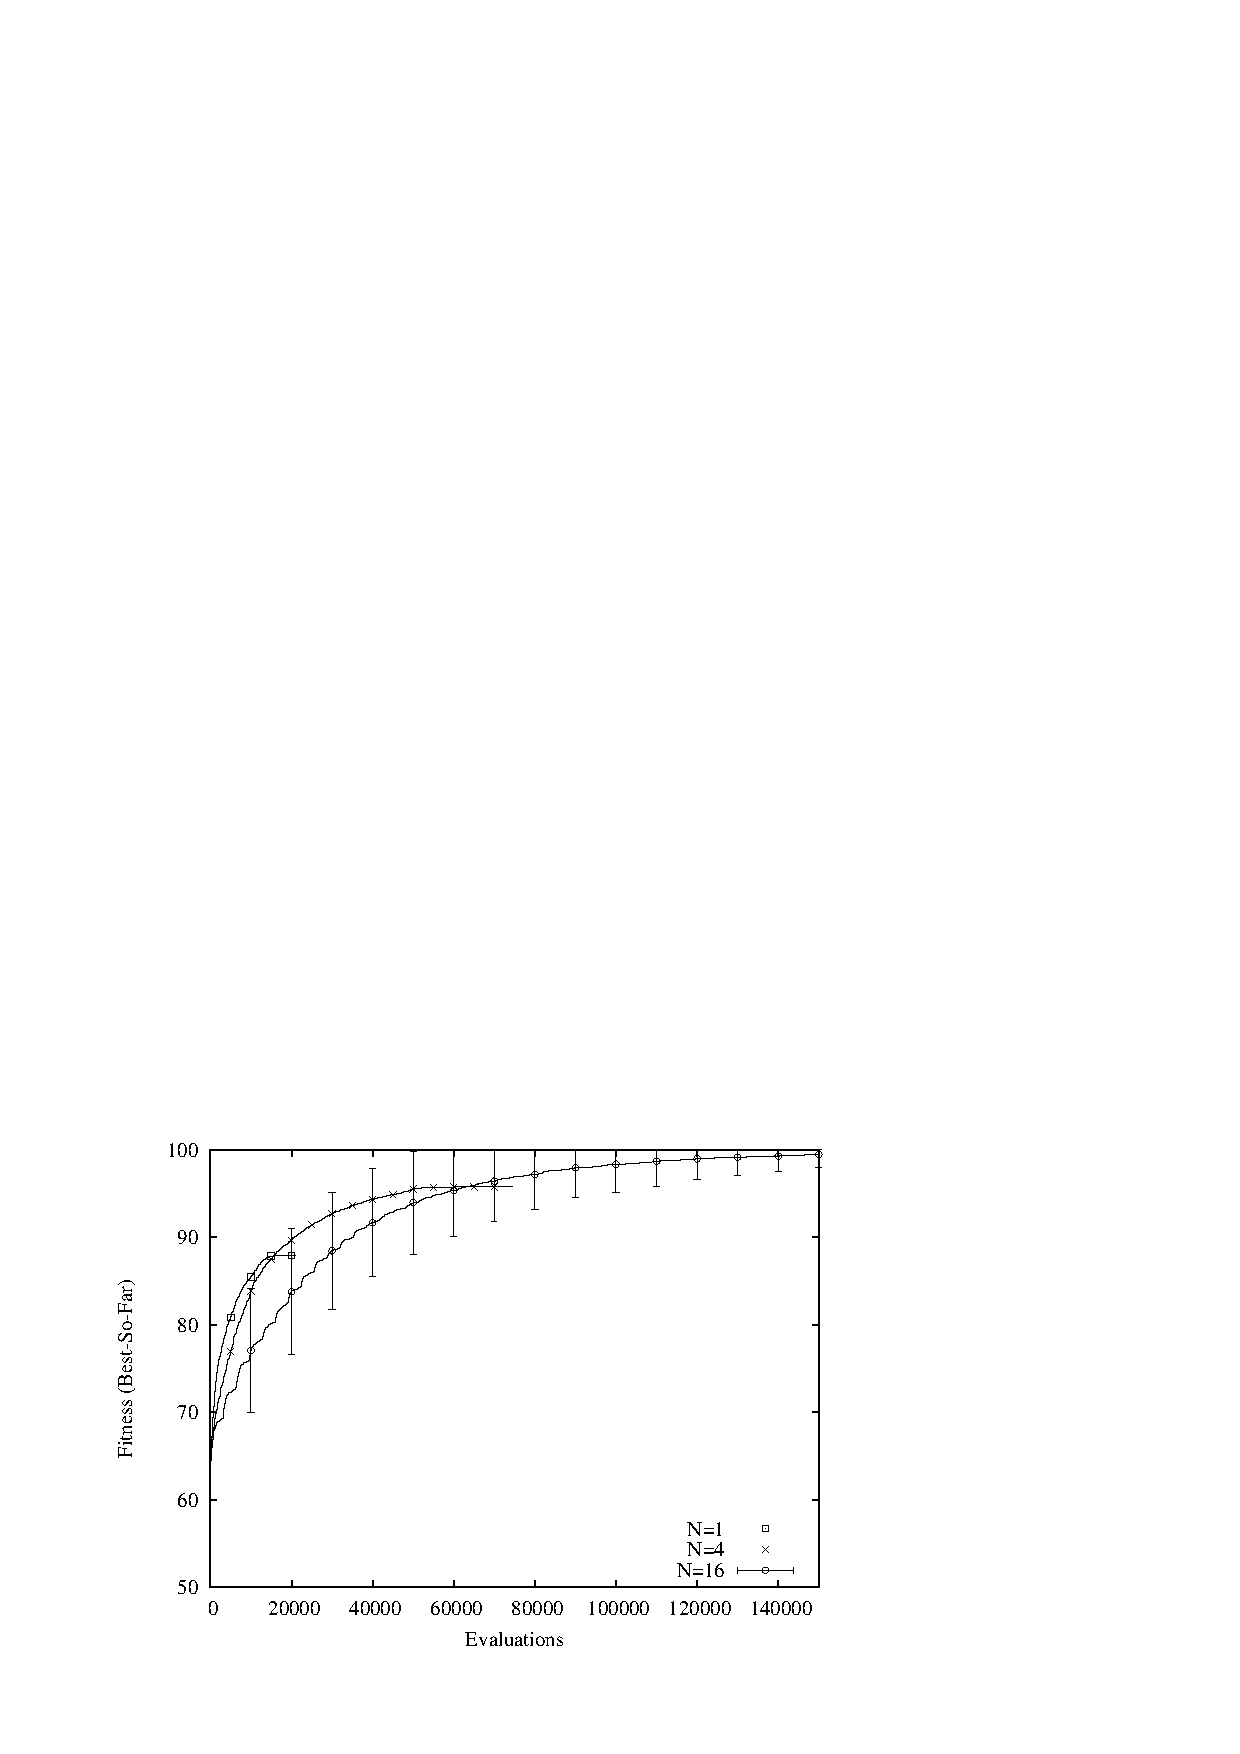
\includegraphics[width=0.9\textwidth]{maxones_cmla_collaborators_alpha_1_evals.pdf}
}

%==========================================================%
% We tried PBIL vs. CEDA on the LOB problem, with not-so-good results for CEDA

\frame{
\frametitle{Some Experiments (PBIL vs. CEDA)}
LeadingOnesBlocks Problem, 100 bits, 5-bit blocks, PBIL 100 samples, $\alpha=0.005$. CEDA $N=8$, $\alpha=1$
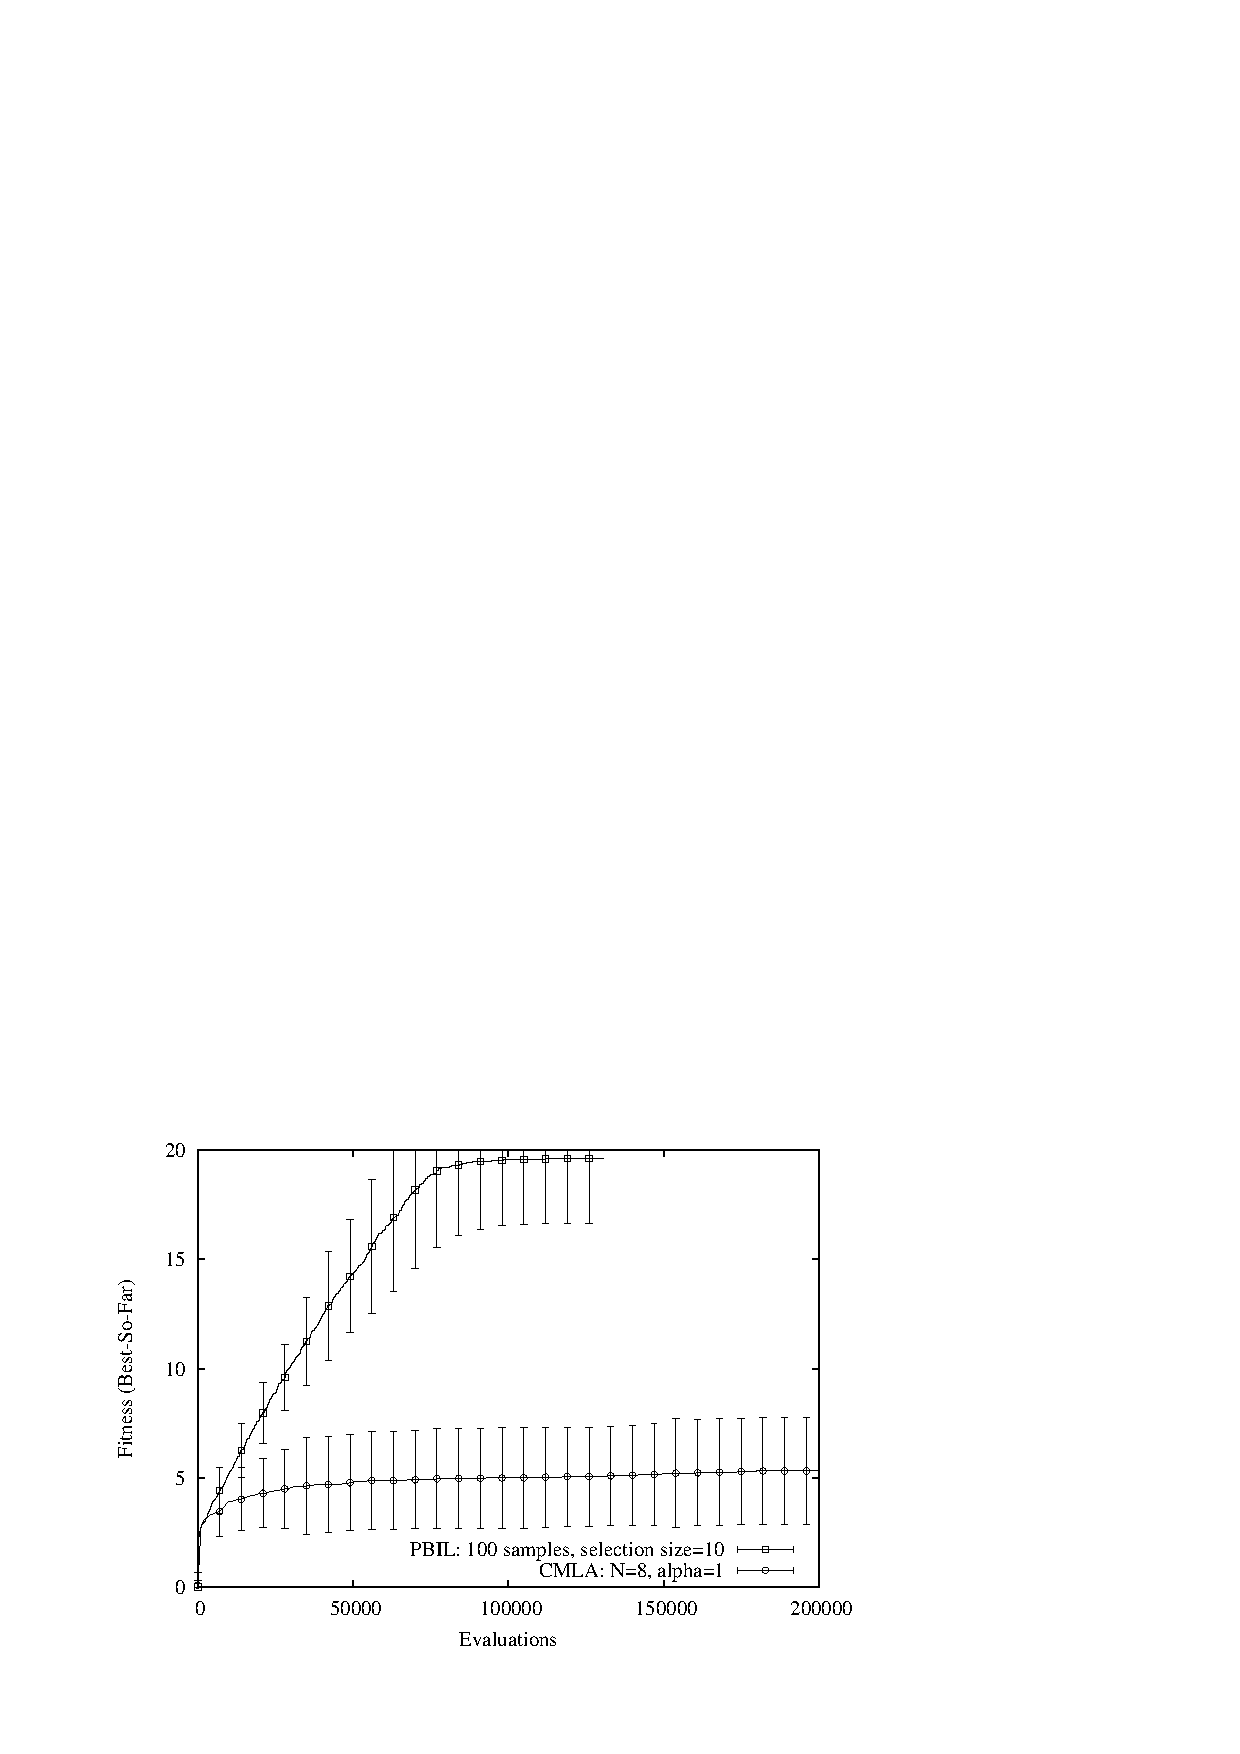
\includegraphics[width=0.9\textwidth]{lobproblem_pbil_vs_cmla_8_alpha_1_evals.pdf}
}

%==========================================================%
% We added PBIL-like alpha to to CEDA and got better results

\frame{
\frametitle{Some Experiments (PBIL vs. CEDA)}
LeadingOnesBlocks Problem, 100 bits, 5-bit blocks, PBIL 100 samples, $\alpha=0.005$. CEDA $N=8$, $\alpha=0.05$
\includegraphics[width=0.9\textwidth]{lobproblem_pbil_vs_cmla_8_alpha_0p05_evals.pdf}
}

%==========================================================%
% Conclusion

\section{Conclusions and Future Work}

\frame{
\frametitle{Conclusions and Future Work}

\structure{Migrating CCEAs \(\longrightarrow\) Univariate EDAs}
\begin{itemize}
\item Can a CCEA algorithm inform an {\it efficient} EDA?
\end{itemize}

\vfill
\structure{Migrating EDAs \(\longrightarrow\) CCEAs}
\begin{itemize}
\item What would a univariate EDA look like in a sample distribution context?
\begin{itemize}
\item How to ``update'' a sample distribution except as an EA?
\item (Obviously boolean EDAs are less interesting here)
\end{itemize}
\item HBOA?
\end{itemize}

\vfill
\structure{Offered for Your Consideration}
\begin{itemize}
\item ACO \(\longleftrightarrow\) A one-population competitive CEA
\end{itemize}

}

%==========================================================%
% Repeated title page

\frame{\titlepage}

\end{document}
